%
The linear phase is succeeded by a transition phase to the saturated phase.
In this phase, the linear modes become large enough for non-linear effects to affect the dynamics of the system.
We will start this chapter by briefly explain how this interaction brings the system into the saturated steady state.

\section{Transition to saturated turbulence}
Through the non-linear terms in the equation (in particular the advective terms) energy from the unstable, growing modes spreads to neighboring modes in the $k$-spectrum.
This can be seen around $t=0.0175\s$ in \cref{fig:fourierUnstable}, where $m_\theta=1$ suddenly shows a growth with a higher growth rate than the rest of the modes.
The transfer of energy can by studied through three-wave coupling under the assumptions that only neighboring modes in the $k$-spectrum interact (the weak turbulence assumption), and that four-wave and higher wave couplings are negligible.
This has been done in for example \cite{Ritz1989,Knorr1990}.

The cascading of energy through the different modes is what eventually brings the system into a saturated turbulence phase.
In an attempt to describe how this happens, an idealized case of fluid turbulence was considered by Kolmogorov and Oboukhov in their $1941$ theory of turbulence \cite{Kolmogorov1962}.
The main assumptions of the theory is that the energy fed into the system in a narrow range of $k$, and that the dissipation of energy only happens at the smallest scales, which in the $k$-spectrum is well separated from the injection of energy.
In other words, there will be a mechanism feeding the turbulence with structures of a certain size.
These structures break up into smaller structures (the energy is cascading to higher $k$), which again break up into smaller structures, all the way until a viscous sink removes the energy from the system.
The famous decay rate $\propto k^{-5/3}$ is then found for the energy through dimensional arguments.

Although the simulated turbulence in our plasma has a more complex turbulent behavior due to more degrees of freedom for the turbulence through the electromagnetic forces, it shares some similarities with the simple fluid picture.
In addition, as mentioned, there exist a big separation the perpendicular and parallel scales in a strongly magnetized plasma.
The perpendicular displacement of fluid parcels is much more restricted than the displacement along the field lines, due to the magnetic field.
Consequently, the turbulence in our simulations have more of $2$-dimensional character than a $3$-dimensional character.

If the enstrophy (global integrated vorticity) is conserved, or at least almost conserved, there can be an inverse cascade of energy (i.e. migration of energy from small scales to large scale), as vortex stretching cannot occur \cite{Fjortoft1953}.
In other words, the eddies will have a tendency to merge together to larger coherent structures.
The main part of the energy, however, is still cascading towards the smaller structures in $2$-D turbulence.
It should be noted that inverse cascades for $2$-D systems has been observed in Earth's atmosphere \cite{Smith2002} in neutral fluid flows, but also arises naturally from the $2$-D Charney-Hasegawa-Mima model \cite{Boffetta2002}, and in the Hasegawa-Wakatani \cite{Manz2009} models in plasma physics.

The turbulence will reach a steady state once the input of energy through the source is balanced by the dissipation of energy.
On the transition from the quasi-linear phase to the turbulent phase a energy overshot is observed (see \cref{fig:energyTrace008}).
%
\begin{figure}[htb]
    \centering
    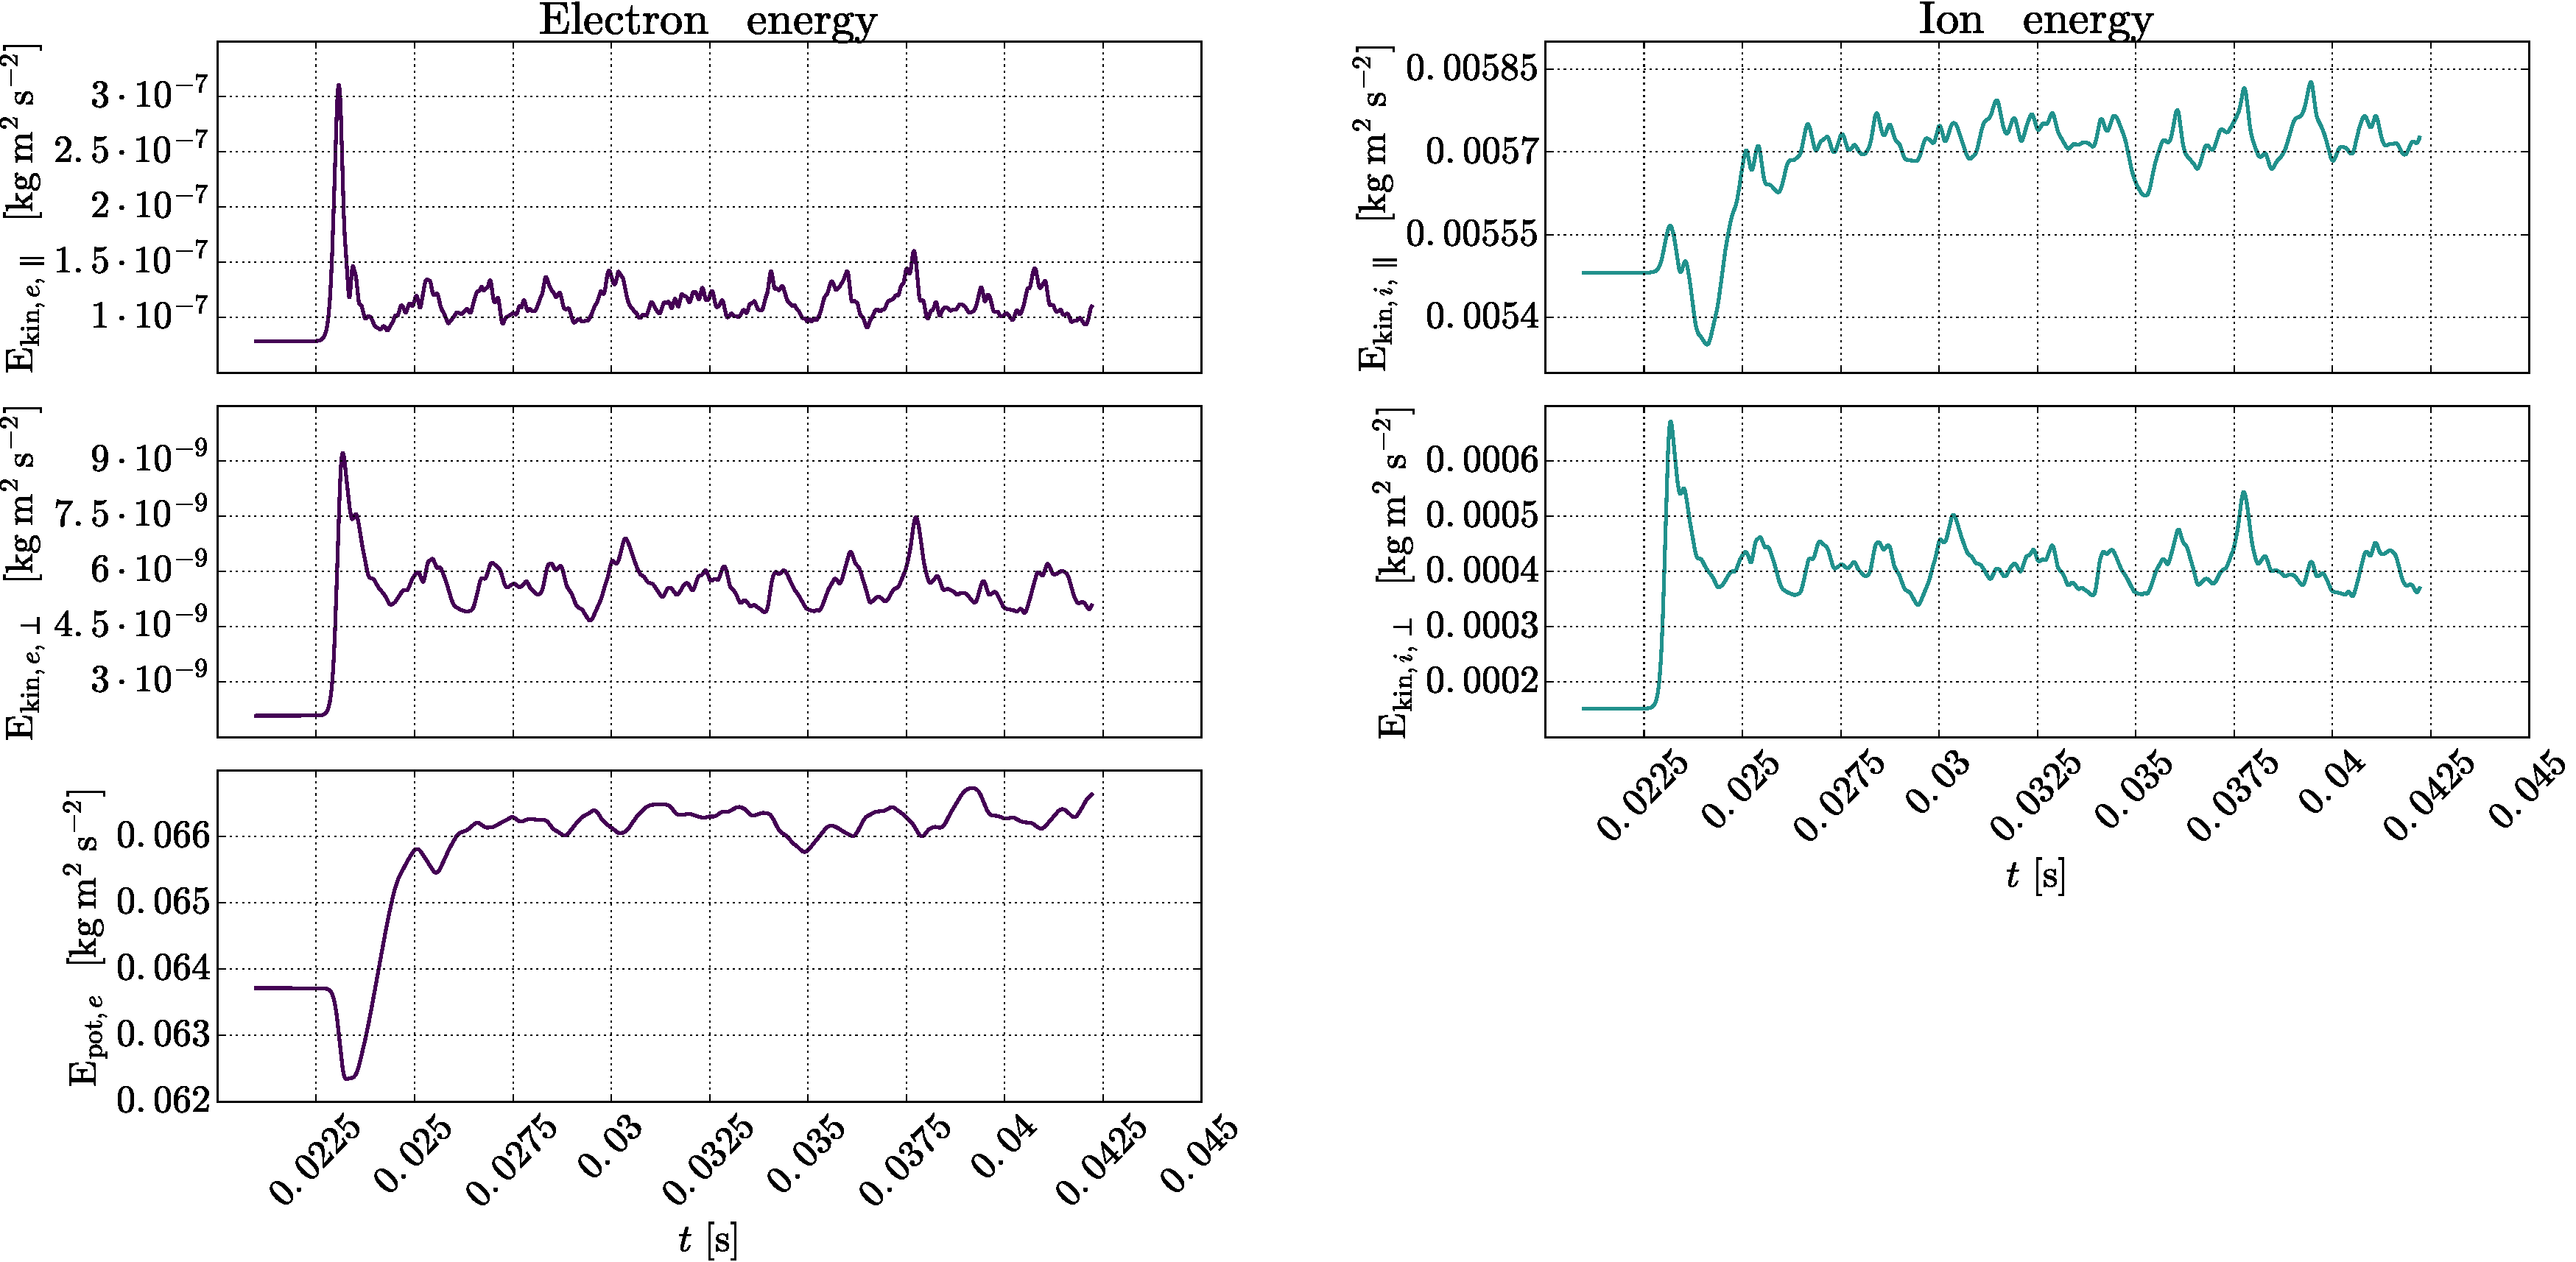
\includegraphics{fig/results/energyTrace/energyTraceB008}
    \caption{Time trace of the energy for $B=0.08\T$.}
    \label{fig:energyTrace008}
\end{figure}
%
As a consequence the eddies evolve at a faster phase at the transition as compared with the saturated turbulent state.
In order to exclude the effects of the transients, we define the start of the saturated turbulence as sometime after the overshoot, around the time where the parallel ion energy is approaching the mean of the rest of the time series.

In the saturated turbulence state, the fluctuations are no longer in an ordered pattern as they were in the linear phase, as shown in \cref{fig:2DFluct}.
%
\begin{figure}[htb]
    \centering
    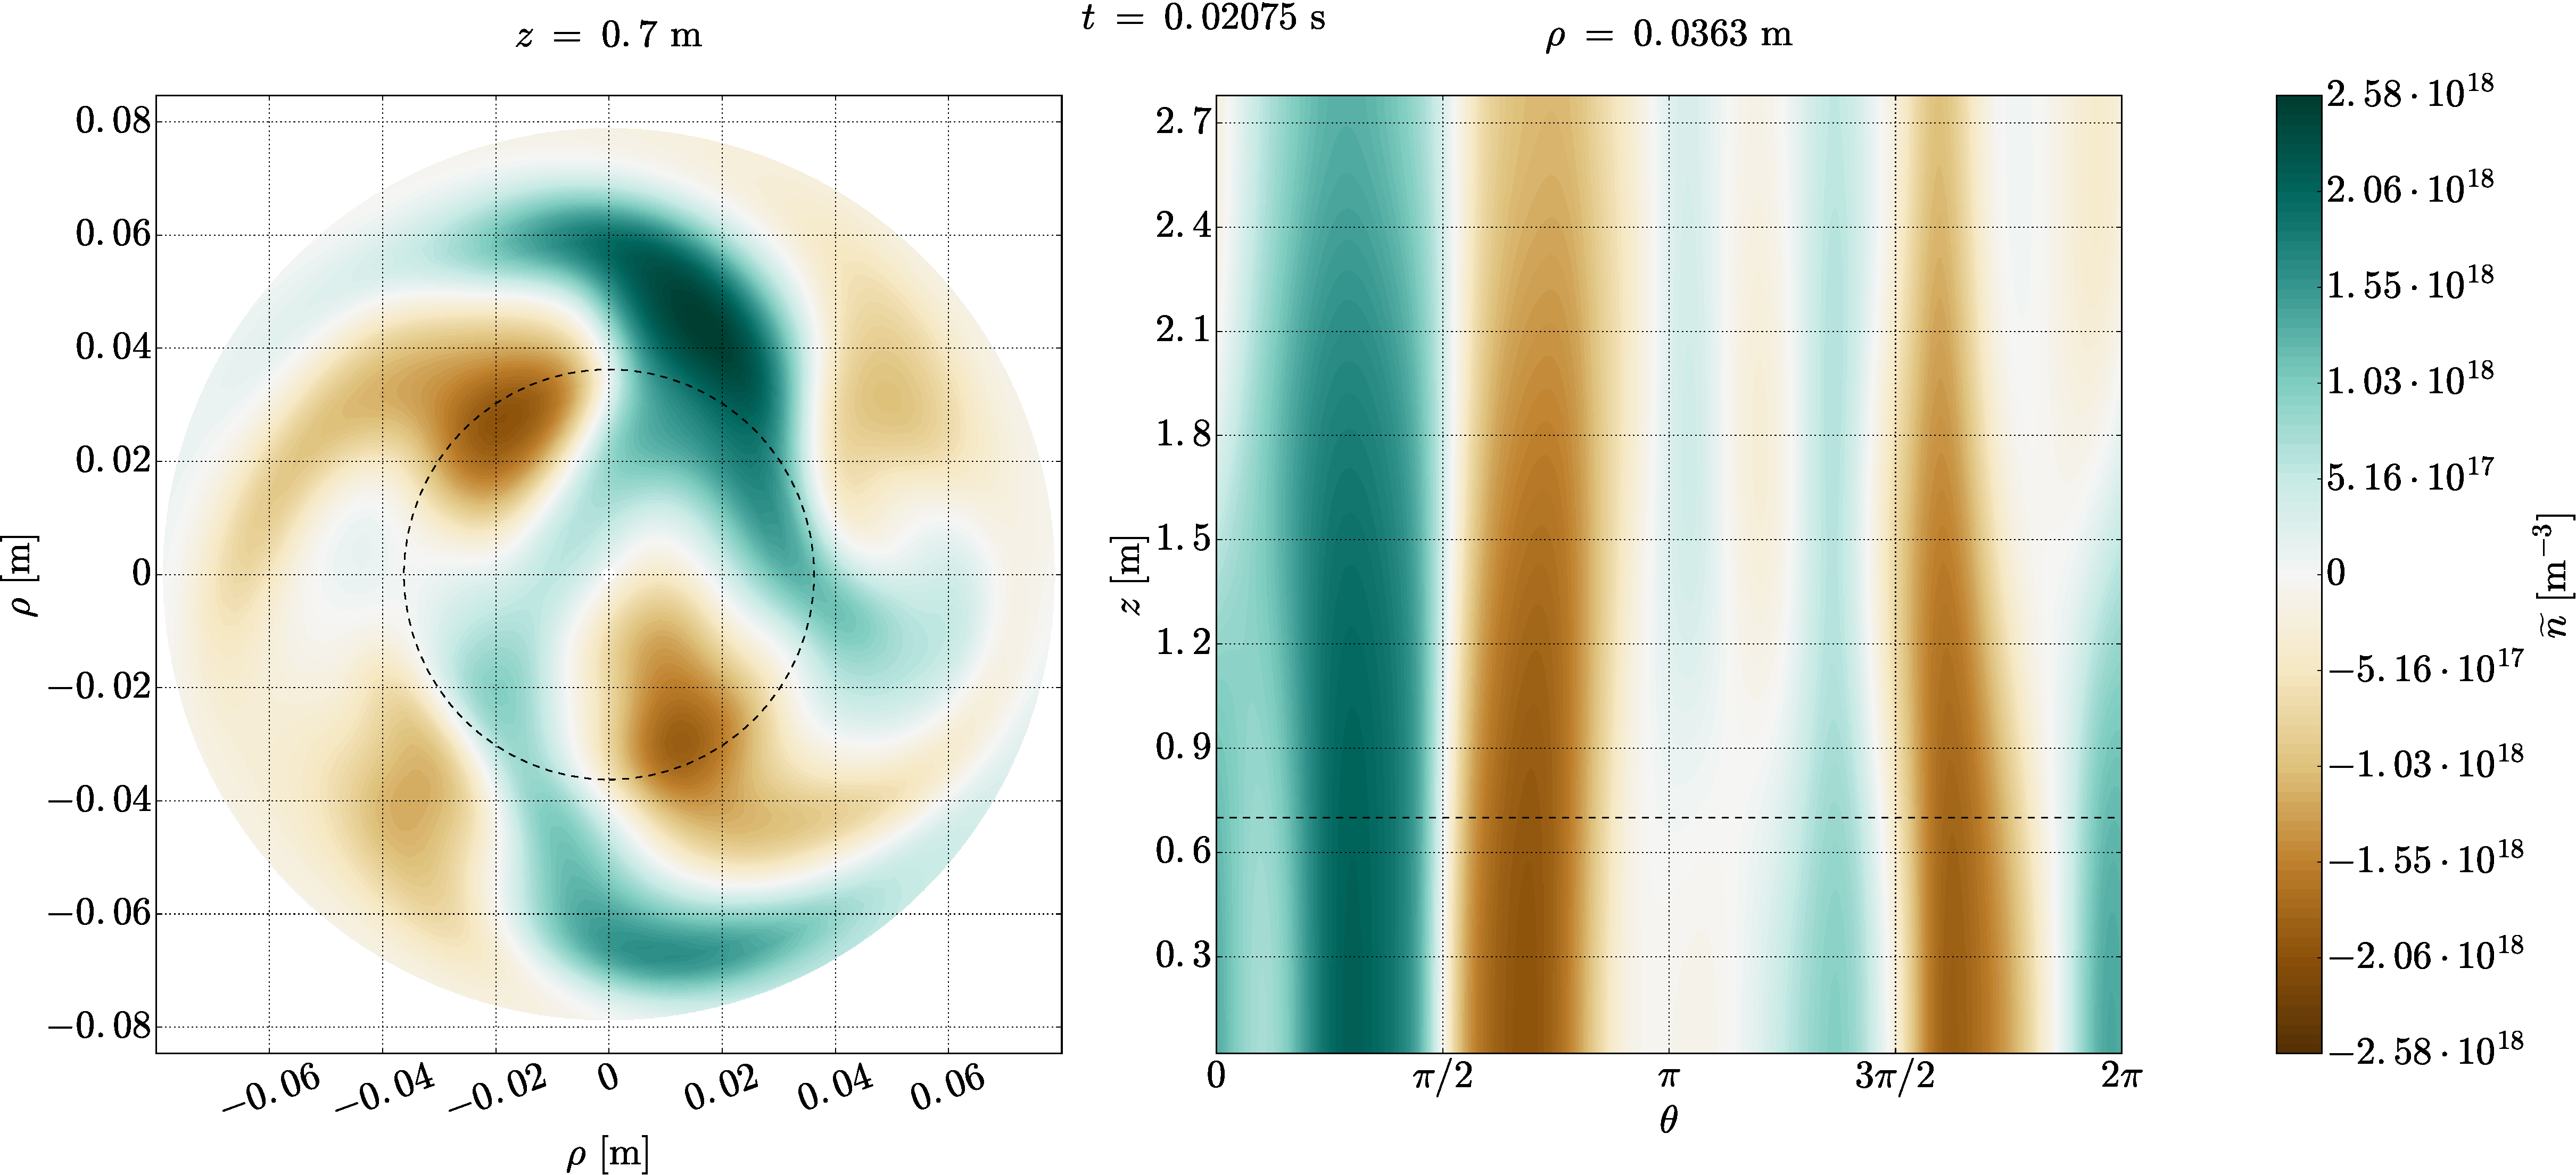
\includegraphics{fig/results/2DTurbulence/fluct}
    \caption{Fluctuations in the turbulent state for $B=0.1\T$}
    \label{fig:2DFluct}
\end{figure}
%
The fluctuations in this state are big enough to push the bulk part of the plasma off-center as observed in the snap-shots of this state in \cref{fig:turbEv}.
%
{
% FIXME: Move this figure and uncomment clearpage and thispage empty when document is done
% \clearpage
% \thispagestyle{empty}
\begin{figure}[htbp]
    \centering
    \begin{subfigure}[h]{1.00\textwidth}
        \centering
        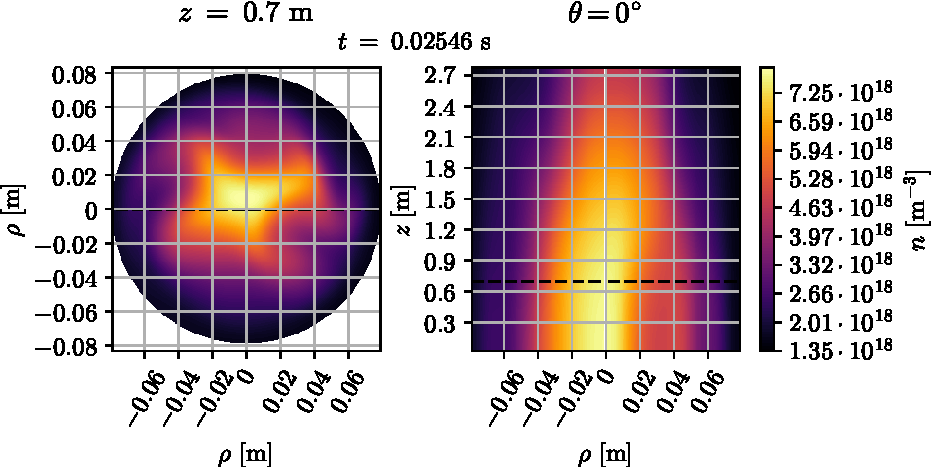
\includegraphics[width=1.0\textwidth]{fig/results/evolution/n-perpPar-2D-0}
    \end{subfigure}%
    \\
    \begin{subfigure}[h]{1.00\textwidth}
        \centering
        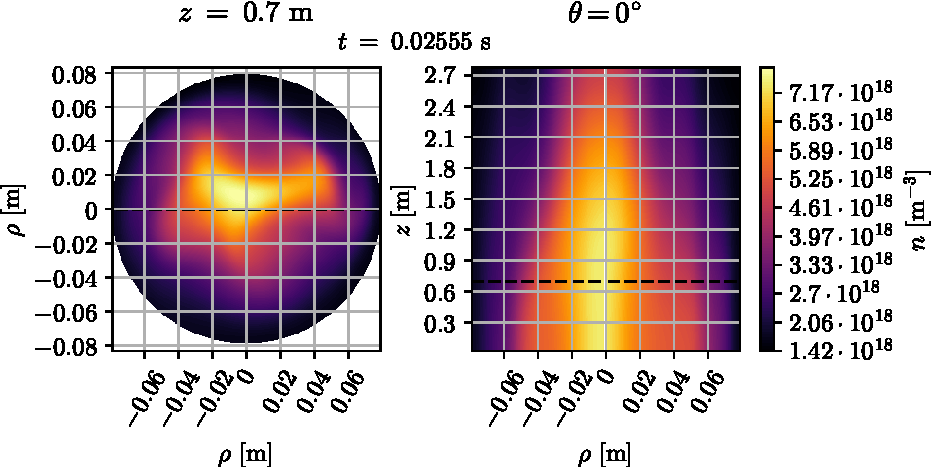
\includegraphics[width=1.0\textwidth]{fig/results/evolution/n-perpPar-2D-1}
    \end{subfigure}
    \\
    \begin{subfigure}[h]{1.00\textwidth}
        \centering
        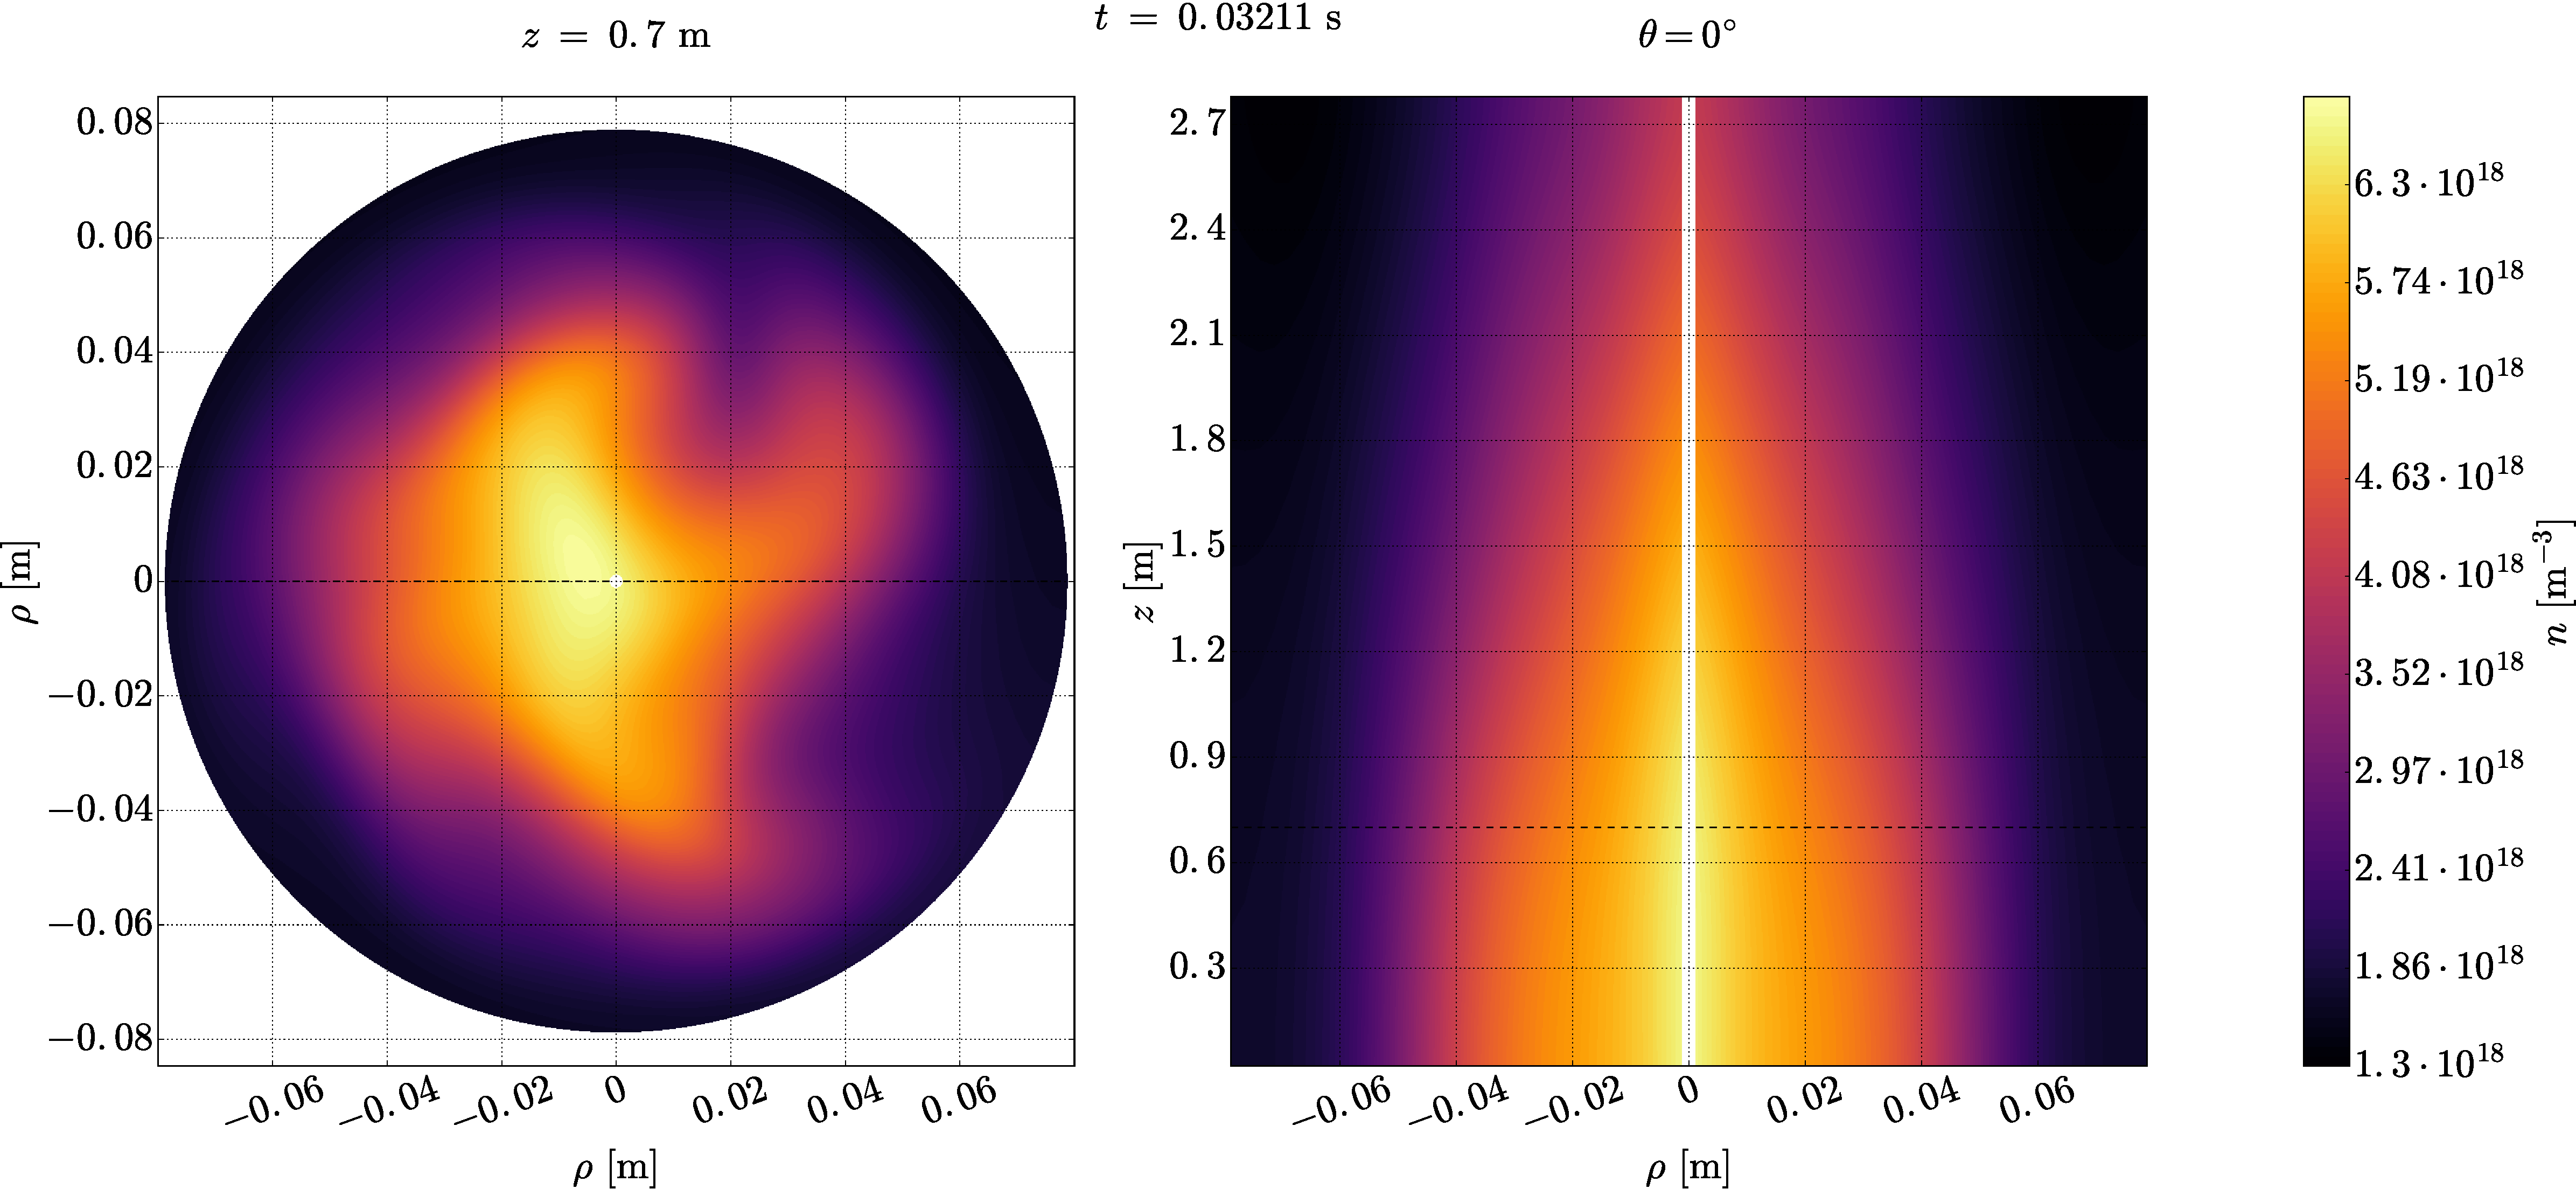
\includegraphics[width=1.0\textwidth]{fig/results/evolution/n-perpPar-2D-2}
    \end{subfigure}
    \caption{Evolution of the plasma in the saturated turbulence phase.
        Here shown for $B=0.08\T$}
    \label{fig:turbEv}
\end{figure}
% \clearpage
}
%

Finally, it is important to note that although there might be one dominating instability which causes the onset to turbulence, the characteristic of the turbulence is more or less independent of the onsetting instability.
In other words, one cannot easily extract the cause of the turbulence by looking at the turbulence alone.
